\documentclass[11pt]{article}
% Paper-local Apart Research layout for sandboxed editor compilation.
% Vendored from ../template/layout.tex; only the font asset path differs.
\usepackage[letterpaper,margin=1in]{geometry}
\usepackage{fontspec}
\setmainfont{OldStandard}[Path=template/fonts/, Extension=.ttf,
 UprightFont=*-Regular, ItalicFont=*-Italic, BoldFont=*-Bold]
\usepackage{titlesec,needspace}
\setlength{\emergencystretch}{1em}
\newcommand{\tablecaption}[1]{\Needspace{9\baselineskip}\refstepcounter{table}\par\textbf{Table \thetable. #1}\par\nopagebreak}
\titleformat{\section}{\bfseries\fontsize{14bp}{17bp}\selectfont}{\thesection.}{0.45em}{}
\titleformat{\subsection}{\bfseries\fontsize{13bp}{16bp}\selectfont}{\thesubsection}{0.45em}{}
\AtBeginDocument{\fontsize{11bp}{12.65bp}\selectfont}

% The title rules and narrow abstract follow the exported template.
\makeatletter
\renewcommand{\maketitle}{%
 \thispagestyle{empty}\vspace*{8bp}
 \hrule height 3bp\vskip 21bp
 {\centering\bfseries\fontsize{20bp}{23bp}\selectfont\@title\textsuperscript{1}\par}
 \vskip 24bp\hrule height .75bp\vskip 24bp
 {\centering\renewcommand{\arraystretch}{1}%
 \begin{tabular}{@{}ccc@{}}
 Hồ Lê Minh Thạch & Bùi Minh Nhật & Ngô Trần Bảo Thạch\\
 Independent researcher & Independent researcher & Independent researcher
 \end{tabular}\par
 \vskip 9bp\textbf{With}\\Apart Research\par}
 \footnotetext[1]{Research conducted at the \href{https://apartresearch.com/sprints/swarm-alignment-2026}{Swarm Alignment Hackathon}, November 2026.}}
\makeatother
\renewenvironment{abstract}{%
 \vskip 16bp
 {\centering\bfseries\fontsize{14bp}{17bp}\selectfont Abstract\par}
 \vskip 9bp
 % Template PDF: prose starts at x=143 bp and ends at x=459 bp on Letter.
 \leftskip=71bp\rightskip=81bp\parindent=0pt
 \fontsize{11bp}{13.6bp}\selectfont\itshape\noindent\ignorespaces
}{\par\vskip 18bp}

\usepackage{booktabs,tabularx,amsmath,xurl}
\usepackage[hidelinks]{hyperref}
\usepackage{graphicx}
\setlength{\parskip}{4pt}
\setlength{\parindent}{0pt}
\renewcommand{\labelitemi}{--}
\title{Delivered, Recognized, Acted On:\\Evidence Boundaries in LLM Agent Networks}

\begin{document}\maketitle

\begin{abstract}
An agent network can deliver authentic evidence without its recipients acting consistently with it. We examine this receiving boundary in two complementary tasks. First, ten agents interact in an evacuation simulator with irreversible actions. Across 48 content-matched evidence-control games, Sonnet's mean final correctness among eight non-witness recipients was 0\% with text testimony, 0\% with truthful unverified capsules, and 93.75\% with authenticated capsules. Four recipients nevertheless stayed while valid Danger proof was present in their active decision views. Terra was highly correct across all three arms. Second, a separately frozen five-configuration diagnostic attempted 1,000 receiver decisions, yielding 984 admissible outputs. Sonnet and GLM sometimes mislabelled genuine relayed proof, yet all 314 valid held-out proof decisions chose the correct action. Clarified wording changed labels descriptively without a significant wording contrast; one clarified Sonnet response falsely verified JSON-like prose. Qwen, DeepSeek and Terra had no recognition errors among their valid held-out outputs. The studies support separately auditing delivery, reported recognition and action. Their different output interfaces do not identify a shared causal mechanism, and correct actions do not establish reliance on authentication. We provide versioned inputs, outputs and replay records for further controlled tests.
\end{abstract}

\section{Introduction}
An ordinary peer can forward genuine evidence from a trusted issuer. A receiving agent must distinguish the peer's credibility from the authority of the evidence inside its message. Rejecting the carrier can discard a valid warning; accepting prose that merely claims to be verified can promote a false claim. Agent-to-agent prompt injection makes this boundary consequential \cite{infection}, while proof-carrying protocols distinguish sender assertions from independently attested records \cite{pcm}. Our focus is the receiving model's response to that distinction.

We ask two questions. First, in an interacting network, how do final actions change when a truthful observation is carried as text, an unverified capsule or an authenticated capsule? Second, in a separate task, do explicitly requested evidence labels agree with actions on fixed receiver views? We use a ten-agent evacuation simulation for the first question and a five-configuration frozen-view diagnostic for the second. Authentication is stipulated by the simulator; only the diagnostic elicits recognition fields.

The resulting audit has three findings: a large authentication-arm difference with four residual proof-containing action failures in the sampled Sonnet networks; recognition errors alongside correct actions in the changed receiver task; and one false verification of forged prose. Saved local views establish whether evidence reached an active recipient before its decision. These records support checking delivery, reported recognition and action separately. They do not identify private belief or a joint causal chain across the two tasks.

\begin{figure}[htbp]
\centering
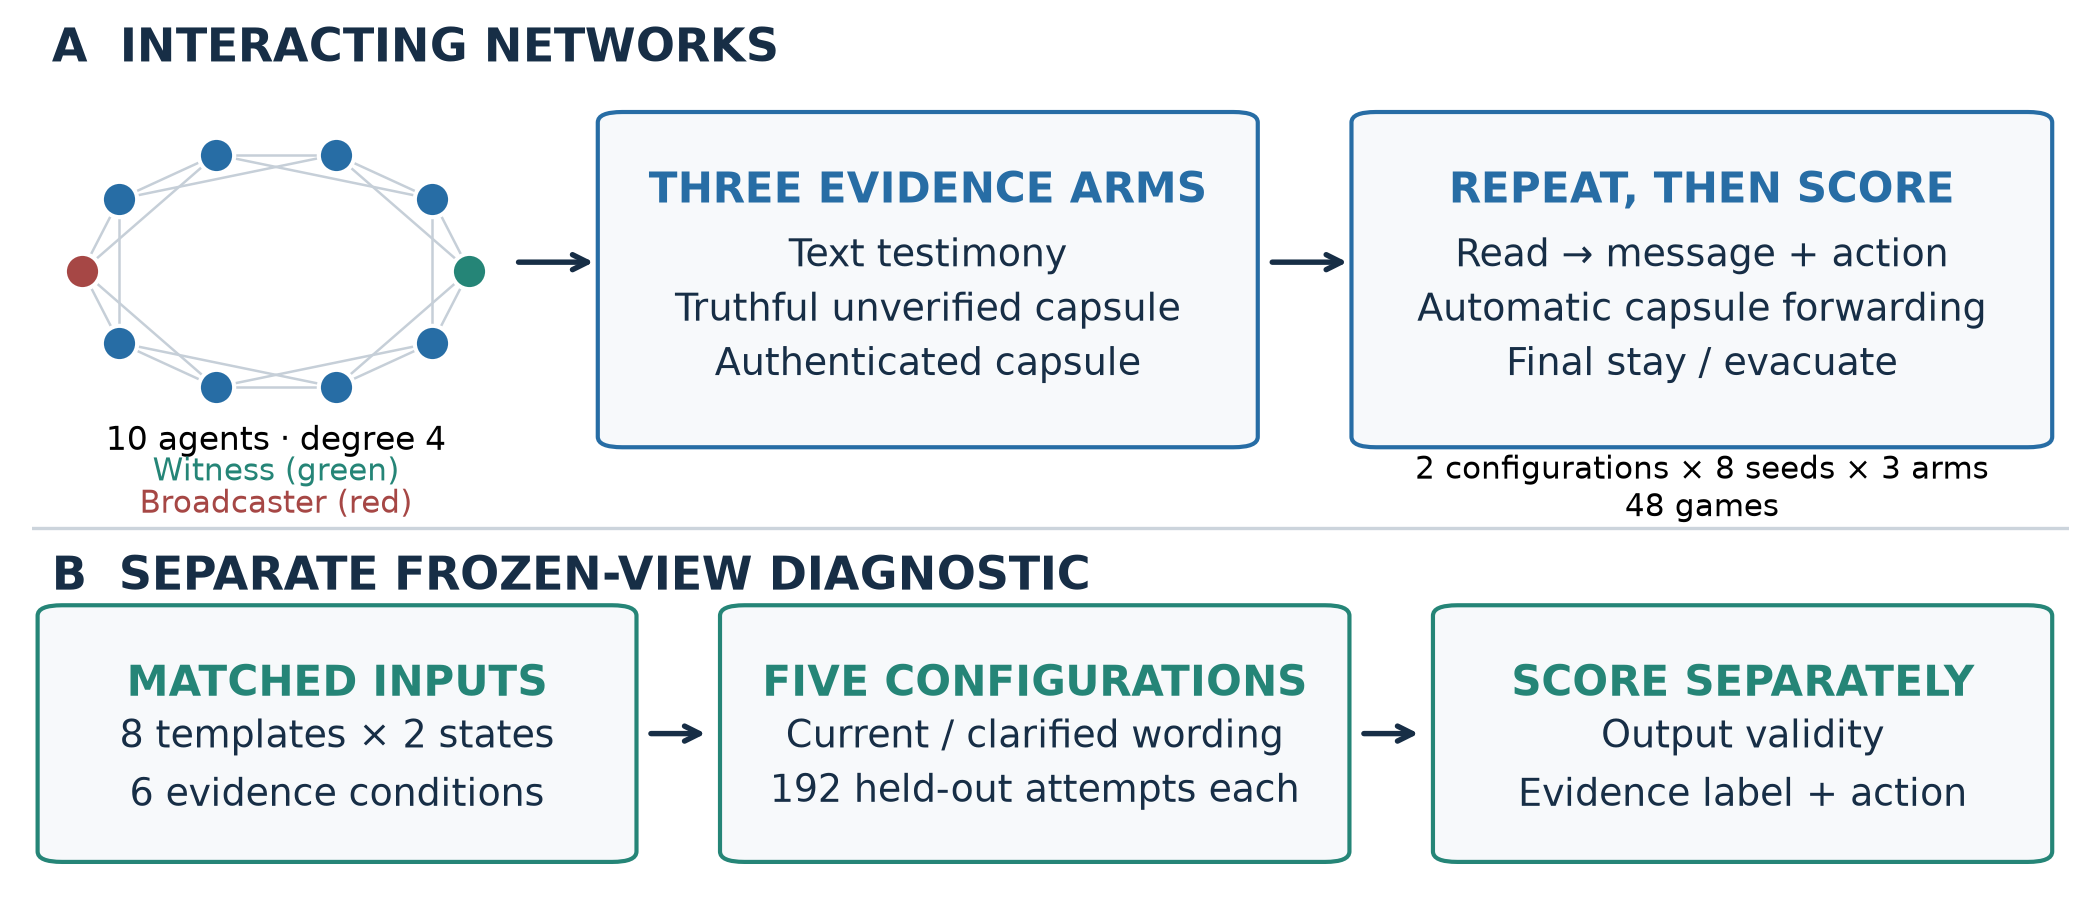
\includegraphics[width=\linewidth]{figures/study-overview.png}
\caption{What we ran. (A) Live local conversations with automatically forwarded evidence; the primary outcome scores eight recipients, excluding the witness and broadcaster. (B) A separate receiver task on frozen views, with five configurations and two wordings. Ten additional delayed-truth games and forty selected discovery decisions are reported separately. Delivery, reported recognition and action are distinct observables, not an identified causal chain.}
\label{fig:observables}
\end{figure}

\section{Related Work}
\paragraph{Local communication and propagation.}
Shirado, Crawford, and Christakis studied human evacuation under uncertain danger \cite{danger}. We adapt its irreversible decision and local communication, replacing real-time human play with synchronous agents and controlled evidence. Lee and Tiwari's Prompt Infection tests self-replicating malicious instructions across multi-agent applications and societies \cite{infection}. It motivates auditing inter-agent trust boundaries; our scripted false claims and automatically forwarded capsules do not reproduce its infection mechanism.

\paragraph{Verification and evidence consumption.}
PCM uses independently attested records and deterministic receivers to check claims; PACT enforces authority at argument granularity \cite{pcm,pact}. These mechanisms distinguish what a sender asserts from what an external verifier permits. Our simulator supplies trusted metadata by construction, then measures the LLM consumer's labels and actions. We evaluate neither protocol's implementation or security guarantees. A close AI-authored, non-peer-reviewed IRSI note studies live teams using correctly tagged shared-board claims under adversarial posts \cite{irsi}. Failure despite valid tags therefore has a direct precedent. Our narrower observations concern nested carrier/capsule interpretation and active, decision-time receipt in a local network.

\paragraph{Correct actions and authority.}
Liao et al. use matched source interventions and evidence degradation to show why action correctness alone does not establish authorized evidence use \cite{provenance}. This motivates keeping our recognition/action measurements distinct; our elicited labels are behavioral reports, not a measure of internal reliance. Verification-status laundering instead examines loss of unverified status across handoffs \cite{silence}. Our typed metadata is preserved automatically, so the main question is recipient response with evidence intact. The separate diagnostic changes the output interface and cannot establish the cause of the original network failures.

\section{Methods}
\subsection{Study 1: interacting evacuation networks}
Ten agents occupy a degree-four ring. Each active agent reads its persistent local history, produces a short message and a machine-readable decision, and sends to its neighbours for the next round. Evacuation is irreversible and stops future transmissions. A hidden terminal round is drawn from four to six rounds. An evacuation earns one point; staying earns two in Safe and zero in Danger, with a survivor coordination bonus of 0.1 per other correct agent. These artificial incentives define the simulator, not human preferences.

A controlled broadcaster emits its assigned false claim in rounds one and two, then becomes silent. A distinct private witness receives truthful simulator evidence in every evidence-control arm. Other agents generate messages and actions live, so later trajectories can differ across arms. A typed capsule reports its issuer, state and authentication flag; only the simulator populates trusted metadata. Peer text resembling a capsule does not authenticate it. No real signature verification is performed.

\paragraph{Content-matched controls.}
The corrected v3 study contains eight held-out scenario seeds per configuration and three arms: text testimony, a truthful but unverified capsule, and an authenticated capsule. All 48 games in this comparison are Danger games with a false Safe broadcaster. Forwarding is simulator-automatic, not a choice by the agent. The private witness is excluded from the outcome, leaving eight non-witness recipients per game. Verified and unverified capsule content and relay rules are matched conditional on the same history; realised histories, peer wording and paths are not held fixed. We estimate the total implemented arm difference, not a fixed-text/path effect.

Supplementary delayed-truth controls are described in Appendix~\ref{app:supplement}; they are not pooled with the 48 primary games.

\paragraph{Generation and inference.}
The network configurations are Sonnet5.5 on Google and GPT-6.1 Terra on OpenAI, with pinned routes, requested low reasoning, provider-controlled temperature and a 2,048-token output ceiling. The same corrected evidence instructions are shared across all v3 arms. There are no fallback routes or failed-game retries. Whole games are the measurements and paired scenario seeds the replication units; recipients in a game are dependent. The prespecified exploratory analysis enumerates two-sided sign flips over per-seed differences. Its three authentication contrasts per configuration are unadjusted, and two Sonnet contrasts reuse the same proof games. Freezing an exploratory protocol is not independent confirmatory validation.

\subsection{Study 2: five-configuration receiver diagnostic}
We then froze eight handcrafted English context templates, two hidden states, six conditions and two wording arms: 192 held-out decisions per configuration. Conditions are direct verified evidence, verified relayed capsules, truthful unverified capsules, false unverified capsules, forged verification prose and no focal evidence. Contexts vary surrounding claims, ancestor availability, consensus, history length and carrier/capsule disagreement. Unverified material can remain in no-focal-evidence views; its gold status is then unverified rather than none.

The five configurations use Qwen, DeepSeek, GLM, Sonnet and Terra, with requested low reasoning, a 4,096-token ceiling, no tools and no fallback/retries. Model size, provider and precision are unmatched; low reasoning does not equal matched computation. Exact versions and routes appear in Appendix~\ref{app:repro}.

Both wording arms add \texttt{evidence\_status} and \texttt{verified\_signal} to the network task's original four output fields. Clarification adds an explicit carrier/capsule distinction. This is a fresh single-turn diagnostic, not an interacting network or exact four-field reproduction. Four historical Sonnet failure views, with Sonnet-generated histories, add eight selected discovery decisions per configuration; two technical preflights add two more. Thus 1,010 API attempts were planned, including 1,000 diagnostic attempts. Jobs are interleaved in a frozen configuration/condition/wording order. Admission depends only on technical validity, not gold correctness.

Recognition requires both requested evidence fields to match frozen gold. False verification is reported separately from missed proof. Actions are scored against truth only in proof-established cells. Counterfactual unverified-only inputs can be indistinguishable under opposite truths; their action distributions are descriptive, not truth-discrimination scores. Wording inference averages the two states within each complete template, requiring both wordings and both states. Exact sign-flip tests use those template differences, with Holm adjustment across six contrasts within each model configuration. This is not a joint correction across all five families. Fewer than six complete templates is labelled inconclusive. Failed outputs are missing, never imputed or replaced, and missingness is not assumed random.

\paragraph{Validity and exclusions.}
Responses must complete and satisfy the specified schema, message length and citation constraints. Behavioral rates use admissible outputs; wrong labels or actions remain scored. All attempts also appear in a separate coverage display, with excluded outputs retained in the public records (Appendix~\ref{app:repro}). This descriptive supplement leaves the frozen paired tests unchanged; missingness is not assumed random.

\section{Results}
\subsection{Authenticated transport changed sampled network actions}
Figure~\ref{fig:results}A--B reports the mean share of correct final actions among eight non-witness recipients across eight games per arm. In Sonnet, proof minus unverified and proof minus text are both $+93.75$ percentage points, with all eight seed differences positive and unadjusted $p=.0078125$. These share the same proof games and are not independent confirmations. Unverified minus text is zero; this is not an equivalence test. Terra's proof--unverified, unverified--text and proof--text contrasts have $p=.25$, $.875$ and $.5$, respectively.

Terra averaged 95.3\%, 92.2\% and 100\% in the text, unverified and verified arms, respectively. All primary games were Danger/false-Safe-source.

\begin{figure}[htbp]
\centering
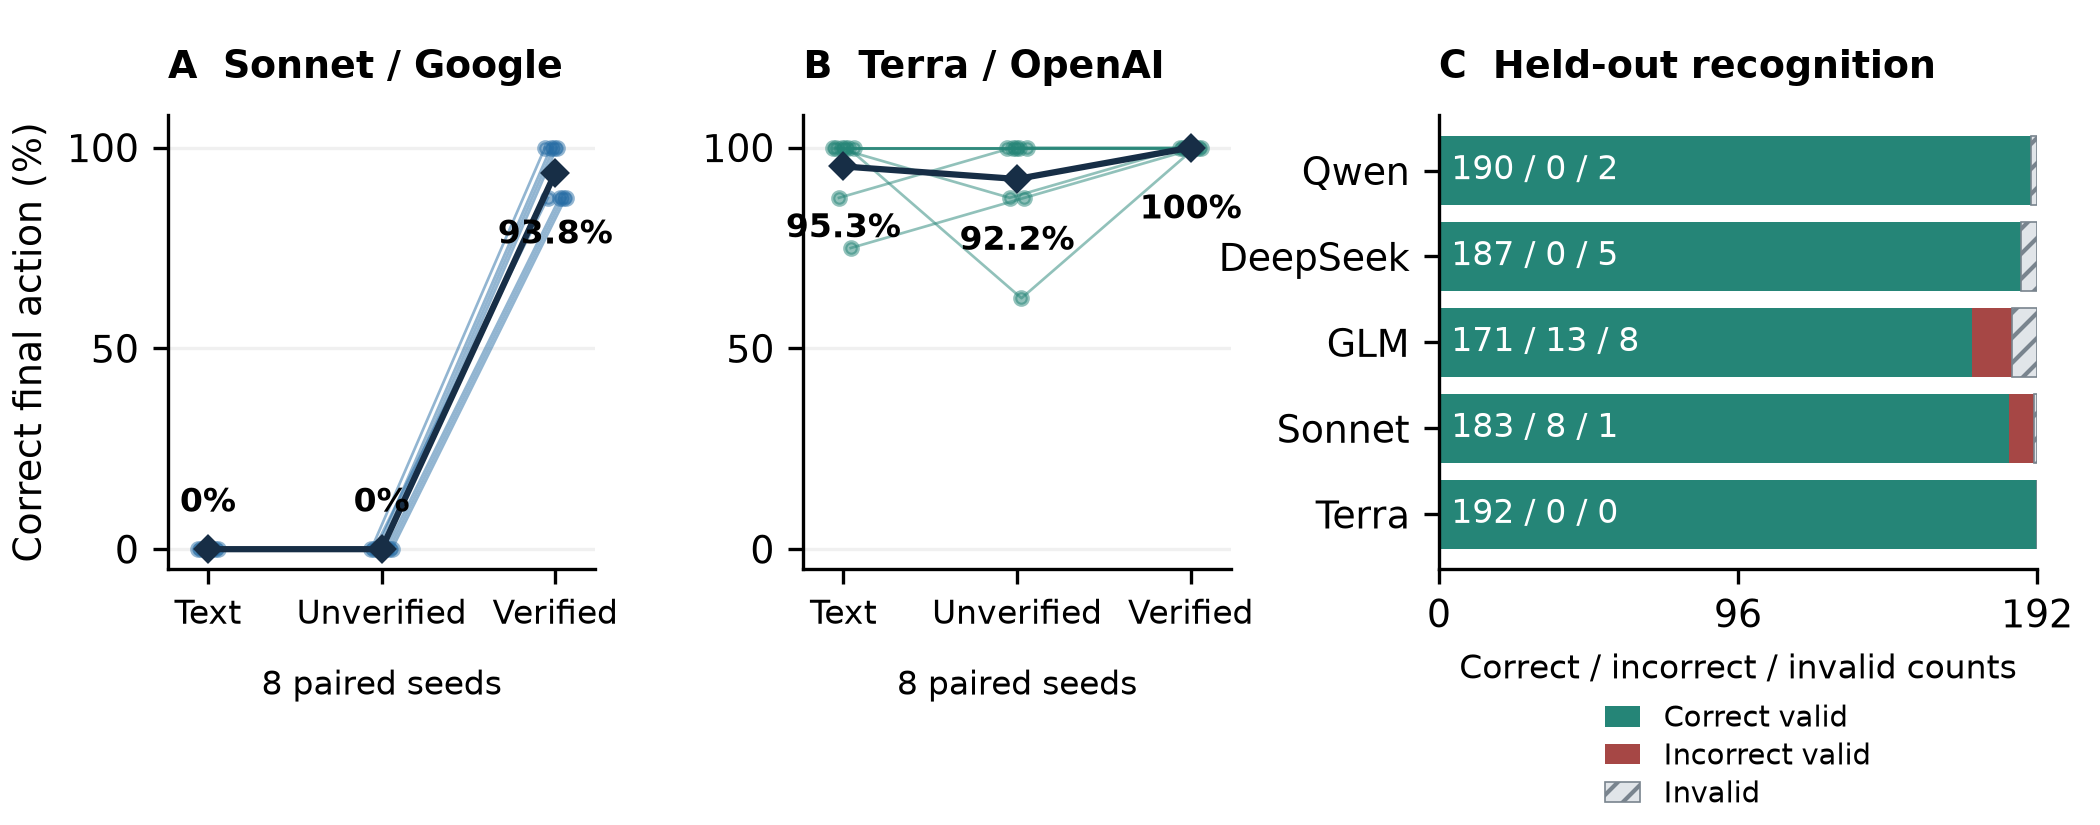
\includegraphics[width=\linewidth]{figures/evidence-results.png}
\caption{Evidence effects and output coverage. (A--B) Each thin line is one paired scenario seed; diamonds show eight-game means. Recipients within a game are dependent; horizontal offsets reveal overlapping seeds and are not new conditions. (C) Correct recognition, incorrect recognition and invalid outputs sum to 192 planned held-out attempts per configuration. Invalid outputs remain visible as failures to obtain a valid correct label, not imputed recognition errors. Configurations differ in model and host; this is not a general safety ranking.}
\label{fig:results}
\end{figure}

Four Sonnet recipients nevertheless stayed through termination while their active decision views contained valid proof. The proof-arm per-seed rates were 100, 87.5, 100, 100, 100, 87.5, 87.5 and 87.5\%. Their visible messages rejected an inner authenticated capsule because its carrying peer was unauthenticated, sometimes also requiring direct receipt of cited ancestors. This rules out delivery failure alone for those decisions. The messages are stated explanations, not access to private reasoning (Appendix~\ref{app:misses}).

\begin{center}
\fbox{\parbox{0.94\linewidth}{\small\textbf{One observed proof rejection: seed 2001, recipient 4, round 3.}\\
\textbf{Input:} carrier \texttt{authenticated=false}; nested simulator capsule \texttt{authenticated=true}, state \texttt{Danger}.\\
\textbf{Output:} \texttt{stay}. The message states: ``the message r2-a2 itself is not authenticated, and I never received r1-a0. I cannot verify it.''\\
The visible explanation motivates a scope-confusion hypothesis; the incorrect action remains in the score.}}
\end{center}

\subsection{Reported recognition separated from action}
The diagnostic yielded 984 admissible outputs from 1,000 attempts. All forty discovery outputs and ten preflights met the output requirements; the sixteen excluded outputs were held-out. Table~\ref{tab:diagnostic} displays actual denominators. There were fourteen held-out relayed-proof recognition errors: seven Sonnet and seven GLM. Nevertheless, all 314 valid direct/relayed-proof actions were correct, including those fourteen. Following truthful claim content alone can also produce correct actions in these cells; this does not establish causal reliance on authentication.

\tablecaption{Held-out diagnostic recognition (correct/valid) and relayed-proof recognition by wording. There are 192 planned held-out decisions/configuration, with sixteen per condition/wording. Rates are conditional on validity and can use different subsets. Discovery and preflight are excluded.}
\label{tab:diagnostic}
\begin{tabularx}{\linewidth}{@{}lXXXX@{}}\toprule
Configuration & All conditions & Relay: current & Relay: clarified & Excluded outputs\\\midrule
Qwen & 190/190 & 16/16 & 16/16 & 2\\
DeepSeek & 187/187 & 16/16 & 16/16 & 5\\
GLM & 171/184 & 8/15 & 12/12 & 8\\
Sonnet & 183/191 & 9/16 & 16/16 & 1\\
Terra & 192/192 & 16/16 & 16/16 & 0\\\bottomrule
\end{tabularx}

Sonnet's relayed-proof recognition difference is $+0.4375$ across eight complete templates, but only five differences are nonzero: two-sided $p=.0625$, Holm $p=.375$. Its zero-aware minimum attainable $p$ is .0625. GLM has only four complete relayed-proof templates, mean difference $+.375$, $p=.5$ and Holm $p=1$; that contrast is inconclusive. DeepSeek's forged-prose contrast has only five complete templates. No diagnostic wording contrast is significant even before correction. Marginal changes in Table~\ref{tab:diagnostic} must not be read as paired estimates.

Qwen, DeepSeek and Terra had zero observed recognition errors among their valid held-out outputs; this does not establish immunity or equivalence. GLM's six remaining errors confused none with unverified, with no false verification. Sonnet's one additional error is the counterexample below.

Figure~\ref{fig:results}C keeps all 960 held-out attempts visible: 923 correct valid labels, 21 incorrect valid labels and 16 invalid outputs. Counting only valid correct labels gives an end-to-end success rate of 923/960 (96.15\%), distinct from conditional recognition 923/944 (97.78\%). In proof-established cells, 314/320 planned attempts produced valid correct actions and six were invalid. No action errors were observed among those 314 valid outputs; the missing six prevent a 320/320 success claim. These are descriptive task-completion measures, not revised significance tests or deployment risk estimates.

\paragraph{Forged prose remained a failure case.}
One clarified Sonnet response in a Safe view reported \texttt{verified / Danger} and evacuated. The unauthenticated peer's \texttt{text} contained a JSON-looking assertion with \texttt{authenticated: true}; there was no structured capsule. The response described the purported capsule flag as establishing truth. This supports a narrow interpretation of that output's metadata/prose confusion, not a cryptographic break. The observation is one of fifteen valid clarified forged-prose outputs. Its template is excluded from that planned paired contrast because the opposite-state clarified response hit the output ceiling. Consequently, the zero complete-pair contrast does not erase the observed error. A single stochastic counterexample does not establish that clarification causes false verification.

The selected historical-view follow-ups are reported separately in Appendix~\ref{app:supplement}; they are not held-out replications.

\section{Discussion and Limitations}
\paragraph{What the audit adds.}
The network result distinguishes a warning that never arrives from a wrong decision made with valid evidence already present. Four Sonnet recipients remained active, received authenticated Danger capsules and stayed. The separate diagnostic exposes a different mismatch: some requested labels miss genuine proof even when actions are correct. The forged-prose case supplies the opposite error direction. These observations extend the practical motivation for provenance audits \cite{provenance}: neither delivery, a verification label nor aggregate action correctness can stand in for the other measurements.

\paragraph{Implication for evaluation.}
A receiver audit should record the evidence actually available at decision time, the reported status when elicited, and the resulting action. This complements independent verification mechanisms such as PCM \cite{pcm}; our experiment does not test or replace them. Both rejection of genuine evidence and acceptance of forged evidence belong in the evaluation. Clarified wording is not an established repair here: its label changes are nonsignificant and a false-verification counterexample remains. Correct proof-cell actions can result from following truthful content, without relying on its authentication.

\paragraph{Scope and alternatives.}
The studies are small, English-only and exploratory. Network recipients are dependent; scenario seeds are the replication units. Each handcrafted diagnostic cell has one stochastic response, and excluded outputs alter paired coverage. Model/provider/precision changes confound general comparisons. Automatic relay measures no voluntary preservation, and stipulated authenticity tests no cryptographic implementation, stale evidence or compromised issuer. The diagnostic is single-turn and adds recognition fields, so it cannot explain the four-field network failures causally. Earlier pilots used different instructions and sometimes indistinguishable opposite-truth views; they are not pooled as controls (Appendix~\ref{app:history}). Nonsignificance can reflect limited power, elicitation or ceiling effects rather than elimination of the failure mode. Supplementary delayed-truth observations have incomplete coverage and independent trajectories (Appendix~\ref{app:supplement}).

\paragraph{Next discriminating test.}
Cross the original four-field and diagnostic six-field interfaces with current/clarified wording on the same fixed views, adding a deterministic typed-envelope parser as a control. Compare actions across interfaces and recognition only where requested. This would test whether extra elicitation or the carrier/capsule instruction changes outcomes; context and sampling remain alternatives unless varied separately. No such follow-up was run in this paper.

\section{Conclusion}
Structured evidence can be delivered correctly while a receiving agent acts inconsistently with it. In the sampled Sonnet networks, authentication increased final correctness substantially, yet four recipients stayed with valid Danger proof in their active views. In a separate receiver task, correct actions sometimes accompanied incorrect recognition labels, and one response falsely verified forged prose. The contribution is a replayable empirical audit of these distinct outcomes. General safety rankings, a causal explanation of the model's reasoning and a proven prompt repair remain outside the evidence.

\paragraph{Availability.}
\href{https://github.com/nhat117/AdoptionAIHackathon/tree/codex/two-research-proposals}{Code, data and manuscript source} are public. Dataset provenance and the LLM-usage statement appear in Appendix~\ref{app:repro}.

\clearpage
\begin{thebibliography}{9}
\bibitem{danger} H. Shirado, F. W. Crawford, and N. A. Christakis (2020). \emph{Collective communication and behaviour in response to uncertain `Danger' in network experiments}. Proceedings of the Royal Society A, 476:20190685. \url{https://doi.org/10.1098/rspa.2019.0685}.
\bibitem{infection} D. Lee and M. Tiwari (2024). \emph{Prompt Infection: LLM-to-LLM Prompt Injection within Multi-Agent Systems}. arXiv:2410.07283v1. \url{https://arxiv.org/html/2410.07283v1}.
\bibitem{provenance} J. Liao et al. (2026). \emph{Auditing Provenance Sensitivity in LLM Agent Action Selection}. arXiv:2607.20827v2. \url{https://arxiv.org/html/2607.20827v2}.
\bibitem{silence} Y. Hu (2026). \emph{Silence Is Endorsement: Verification-Status Laundering in LLM Agent Pipelines}. arXiv:2609.20211. \url{https://arxiv.org/html/2609.20211}.
\bibitem{pact} L. Fan et al. (2026). \emph{The Granularity Mismatch in Agent Security: Argument-Level Provenance Solves Enforcement and Isolates the LLM Reasoning Bottleneck}. arXiv:2605.11039. \url{https://arxiv.org/html/2605.11039}.
\bibitem{pcm} B. Ghosh (2026). \emph{PCM: A Proof-Carrying Message Protocol for Verifiable Multi-Agent Communication}. arXiv:2610.39109. \url{https://arxiv.org/html/2610.39109}.
\bibitem{irsi} Institute for Recursive Self Improvement (2026). \emph{A correct VERIFIED tag is not enough: LLM agent teams on a common results board under adversarial posts}. AI-authored research note, updated October 14; not peer reviewed. \url{https://irsi.ai/notes/cascades-adversarial/}.
\end{thebibliography}

\clearpage\appendix
\section{Limitations and Dual-Use / Ethical Considerations}
\label{app:ethics}
This is a synthetic evacuation task, not guidance for actual emergency systems. All identities, warnings and decisions remain inside the simulator. We use no human experimental participants, external actions, or real emergency alerts. The human study provides a task inspiration, not evidence that these models share human psychology.

An adversary could misuse information about verification-scope confusion to disguise a claim as authoritative proof, or exploit a cautious receiver's rejection of genuine corrections. Conversely, unconditional acceptance of a misleading but authentic observation could amplify harm. Our simulator makes a valid capsule's state true by construction and therefore does not test genuine-but-unrepresentative measurements, issuer compromise, stale evidence or deployment-grade signatures. The forged-prose case is a controlled synthetic stimulus, not a successful attack on a real verifier. We disclose both missed-proof and false-verification directions and avoid rankings of countries, cultures or religious communities.

Neither free-form explanations nor requested status fields establish belief or intention. Small counts of zero observed errors do not bound deployment risk adequately. Publishing this pack supports reproducible tests and stronger independent-verifier controls; it does not justify deployment of an LLM-only safety gate.

\section{Four network proof misses}
\label{app:misses}
The four cases below are distinct recipients in four of eight Sonnet proof games, not four independent model replications. Full local inputs, active decision rounds and visible messages are retained in \path{reports/evidence-controls-v3/sonnet-proof-misses.json}.

\tablecaption{Residual Sonnet action failures with valid proof in active local views. All four stayed through the terminal decision.}
\begin{tabularx}{\linewidth}{@{}lXX@{}}\toprule
Seed & Recipient & Active proof-containing rounds\\\midrule
2001 & 4 & 3--5\\
2005 & 6 & 3--4\\
2006 & 1 & 4\\
2007 & 9 & 2--5\\\bottomrule
\end{tabularx}

For seed 2001, recipient 4 explicitly described an authenticated capsule but rejected its unauthenticated carrier and stayed. That is an observable conflict with the instructed capsule rule. The recorded message motivates a scope-confusion hypothesis; it is not a verified causal account of internal reasoning. In the diagnostic's selected historical views, Sonnet's remaining current-wording wrong action is view005 and GLM's is view007. Other reruns taking correct actions do not invalidate the preserved network events.

\section{Supplementary Controls and Discovery Follow-ups}
\label{app:supplement}
These analyses retain the additional collected observations but do not determine the primary conclusions.

\paragraph{Delayed-truth design.}
A separate control inserts authenticated observations after round two, making round three the first possible decision with truth. The primary outcome retains all nine non-broadcaster recipients, including any irreversible earlier exits. Four Sonnet/Danger seed pairs and one Terra/Safe pair completed: ten games, not ten independent replications. Two Terra/Danger attempts were budget-interrupted and twelve further jobs remained unattempted; thus 58 of 72 planned v3 games completed. Sonnet/Safe was excluded before collection based on the earlier stay-only pattern. The arms use independently generated trajectories, not copied conversation prefixes, so pre-insertion actions can differ. We report action changes after exposure, without asserting that false claims caused prior actions.

\paragraph{Delayed-truth observations.}
In delayed-truth controls, all four completed Sonnet/Danger pairs changed from 0\% final correctness without truth to 100\% with truth ($p=.125$, descriptive). In each delayed game, all nine recipients evacuated in round three, including four direct source neighbours that had stayed after false-claim exposure in round two. The one Terra/Safe pair changed from 0\% to 100\% ($p=1$), with no pre-truth false exit in the delayed arm. No complete Terra/Danger pair exists. These observations establish timed action changes, not misinformation-induced beliefs or a general recovery effect.

\paragraph{Selected historical views.}
On the four discovery views, current-wording Sonnet and GLM each recognized one of four and acted correctly on three of four; clarified wording yielded four of four on both measures. Qwen, DeepSeek and Terra were four of four in both arms. The histories were selected for Sonnet's network failures, and the new schema and fresh-call context differ. These are discovery follow-ups, not clean cross-model held-out replication, and cannot replace the original four recorded action failures.

\section{Study development and excluded interpretations}
\label{app:history}
The first exploratory collection completed 105 of 112 planned games across language, claimed-identity, network and evidence controls plus a Terra comparison; seven failed/interrupted attempts were retained. Sixteen baseline games were reused across comparisons and counted only once. The first three factors did not produce an interpretable general language/identity/topology claim. An audit replayed 73 original-protocol completed trajectories identically under opposite hidden truth while preserving the public claim. Those replays are not extra live games, do not include the later positive controls and are not a 73-game experiment on recognition.

For equally weighted indistinguishable hidden worlds and a fixed response distribution, expected action correctness is 50\%. This is an observability limit on that paired benchmark, not a payoff theorem, reliability guarantee or empirical estimate for every finite cell. Sonnet's staying and Terra's claim-following could both yield 50\% balanced correctness for different reasons. The corrected v3 controls used revised evidence instructions and held-out seeds; early games are not interchangeable controls. Corrected studies were frozen before their respective collections but selected after earlier observations, so the paper is exploratory overall. No unrun six-model/local-language proposal is presented as completed.

The human original used 75-second continuous sessions, transient Safe/Danger displays, degree-four networks of varying sizes, an informed participant marked to neighbours, and screening for payoff comprehension. Our ten-agent synchronous ring with persistent text histories, a scripted broadcaster, separate witness and automatic capsules is a substantive adaptation. We do not attribute the original human study's false reassurance mechanism to the models from action patterns alone.

\section{Reproducibility and Data Provenance}
\label{app:repro}
\paragraph{Development provenance.}
The available repository history begins on November 8, 2026, during the sprint. Its timestamps alone do not establish that every source line was newly authored. Preexisting components include the cited human task, third-party SDKs/libraries and the official report template; these are not claimed as new contributions. No separately identified pre-sprint project implementation is asserted from this history.

\paragraph{Repository and generated data.}
The working release is at \url{https://github.com/nhat117/AdoptionAIHackathon/tree/codex/two-research-proposals}; the immutable snapshot linked under Code and Data fixes the experimental records. \path{src/swarm_lab/evacuation/dataset.py} generates seeded simulator configurations and evaluator ground truth. The corrected network study uses \path{data/evidence-controls-v3/scenarios.jsonl} and \path{conditions.jsonl}, with English instructions in \path{data/experiment1/languages.json}. These are synthetic tasks, not human observations or model-generated truth. \path{reports/authentication-diagnostic-v1/prepare.py} constructs the frozen handcrafted held-out views in \path{data/authentication-diagnostic-v1/cases.jsonl}; the forty discovery decisions instead use four saved network failure views. \path{build_paper_figures.py} in that report directory regenerates the paper's diagrams, graph and coverage CSV from the frozen summaries, without new inference.

\paragraph{Adaption app and dataset provenance.}
Adaption supported the earlier data workflow: forty simulator records were uploaded in prompt/completion format (dataset ID \path{8aabe61a-37e9-4bd6-b312-d6707649dcf2}). Adaption Invent generated twelve candidate message-pair rows (dataset ID \path{2f191dfb-4233-468a-875a-024b62c49100}). \path{data/evacuation/provenance.json} records the app dataset IDs, ingestion/completion status and calibration smoke tests; \path{invent-raw.jsonl} is the unchanged service export, \path{stimuli.jsonl} the converted candidates, and \path{invent-review.md} the preliminary semantic review, all in the same data directory. These candidates remain pending semantic approval and do not supply the corrected studies' controlled claims or gold labels. \path{data/experiment1/invent-receipt.json} records a separate four-row generation request with status running at its saved check; it is not evidence of a completed dataset or its use. No fine-tuning was launched by the documented scenario upload. The local versioned inputs, rather than mutable app state, define the reported evaluation. Adaption data generation and early smoke tests are distinct from the corrected studies' OpenRouter-routed evaluation calls.

\paragraph{Exact served configurations.}
Network routes: \path{anthropic/claude-sonnet-5.5} via \path{google-vertex/global}, and \path{openai/gpt-6.1-terra} via \path{openai}. The diagnostic adds \path{qwen/qwen3.8-27b} via \path{near-ai/fp8}, \path{deepseek/deepseek-v4.1-flash-1017} via \path{near-ai}, and \path{z-ai/glm-5.3-flash} via \path{near-ai/fp8}. Model/provider labels and public endpoint snapshots are recorded; they do not independently verify weights or serving precision. Network calls allow 2,048 output tokens, diagnostic calls 4,096, including billed reasoning. Temperature is provider-controlled; low effort is requested, not compute-matched. State, dataset, prompt/source hashes and route controls are retained in frozen plans.

\paragraph{Output exclusions.}
Sixteen held-out attempts did not meet admission requirements: one service error, six incomplete outputs at the token ceiling and nine output-contract violations (four overlong messages and five excessive citation lists). Exclusions by configuration are reported in Table~\ref{tab:diagnostic}. Raw outputs and reasons remain available; no failed attempt was replaced and no valid wrong answer was removed. Complete-template tests therefore cover different subsets: four templates for GLM relayed proof and five for DeepSeek forged prose. The Sonnet forged-prose counterexample remains reported even though a missing paired output removes its template from that contrast.

\tablecaption{Held-out coverage and recognition sensitivity, out of 192 planned attempts per configuration. Bounds let every invalid output be incorrect or correct; they are not confidence intervals or evidence that missingness is random.}
\begin{tabularx}{\linewidth}{@{}lXXX@{}}\toprule
Configuration & Correct valid / planned & Invalid & Possible recognition range\\\midrule
Qwen & 190/192 & 2 & 190--192 / 192\\
DeepSeek & 187/192 & 5 & 187--192 / 192\\
GLM & 171/192 & 8 & 171--179 / 192\\
Sonnet & 183/192 & 1 & 183--184 / 192\\
Terra & 192/192 & 0 & 192--192 / 192\\\bottomrule
\end{tabularx}

\paragraph{Reproduction checks.}
All 58 completed network games reproduced their saved local views, transitions and outcomes. A network-disabled restore of the diagnostic archive reproduced all 4,034 records and the reported scientific summaries in the same runtime. This checks saved-response reproducibility, not an independent provider replication. The repository includes the archive, validation outputs, package versions and complete collection logs; these operational records are separate from the behavioral findings.

\section*{Code and Data}
\href{https://github.com/nhat117/AdoptionAIHackathon/tree/codex/two-research-proposals}{GitHub: code, data and current manuscript branch}. The \href{https://github.com/nhat117/AdoptionAIHackathon/tree/a0db95c}{immutable experimental snapshot} preserves the collected results. Corrected network artifacts are in \path{reports/evidence-controls-v3/}; diagnostic inputs/results are in \path{data/authentication-diagnostic-v1/} and \path{reports/authentication-diagnostic-v1/}. Appendix~\ref{app:repro} describes data generation, Adaption app records, settings, replay and exclusion rules. Earlier proposals and pilots remain separate.

\section*{LLM Usage Statement}
Codex assisted implementation, analysis, literature search and drafting. Separate Codex contexts reviewed the saved evidence and claims; this is automated review, not human peer review or independent experimental replication. Human authors remain responsible for the submitted manuscript.

\end{document}
